\section{Waterfall}
A fundamental aspect to the waterfall model is the fact that the project is 
expected to progress down the primary path \citep{sergei:2012:Online}. The 
primary path is the most commonly used path through out a system. By 
highlighting the primary path, the major processes and tasks are easily mapped
out, a clear indication of what exactly is required to be completed.

The waterfall model contains six main phases --- requirements analysis, 
specification, design, coding, testing and implementation \citep{dawson09}. 
Deliverables are achieved as the flow down the primary path is completed. 

It is possible however for a reverse flow. This reverse flow represents a 
change applied to a prior deliverable, which was only recognised in the 
deliverable after the change is required in. This is known as rework, and can 
result in both the current deliverable and previous deliverables to be 
repeated.

\begin{figure}[H]
  \centering
  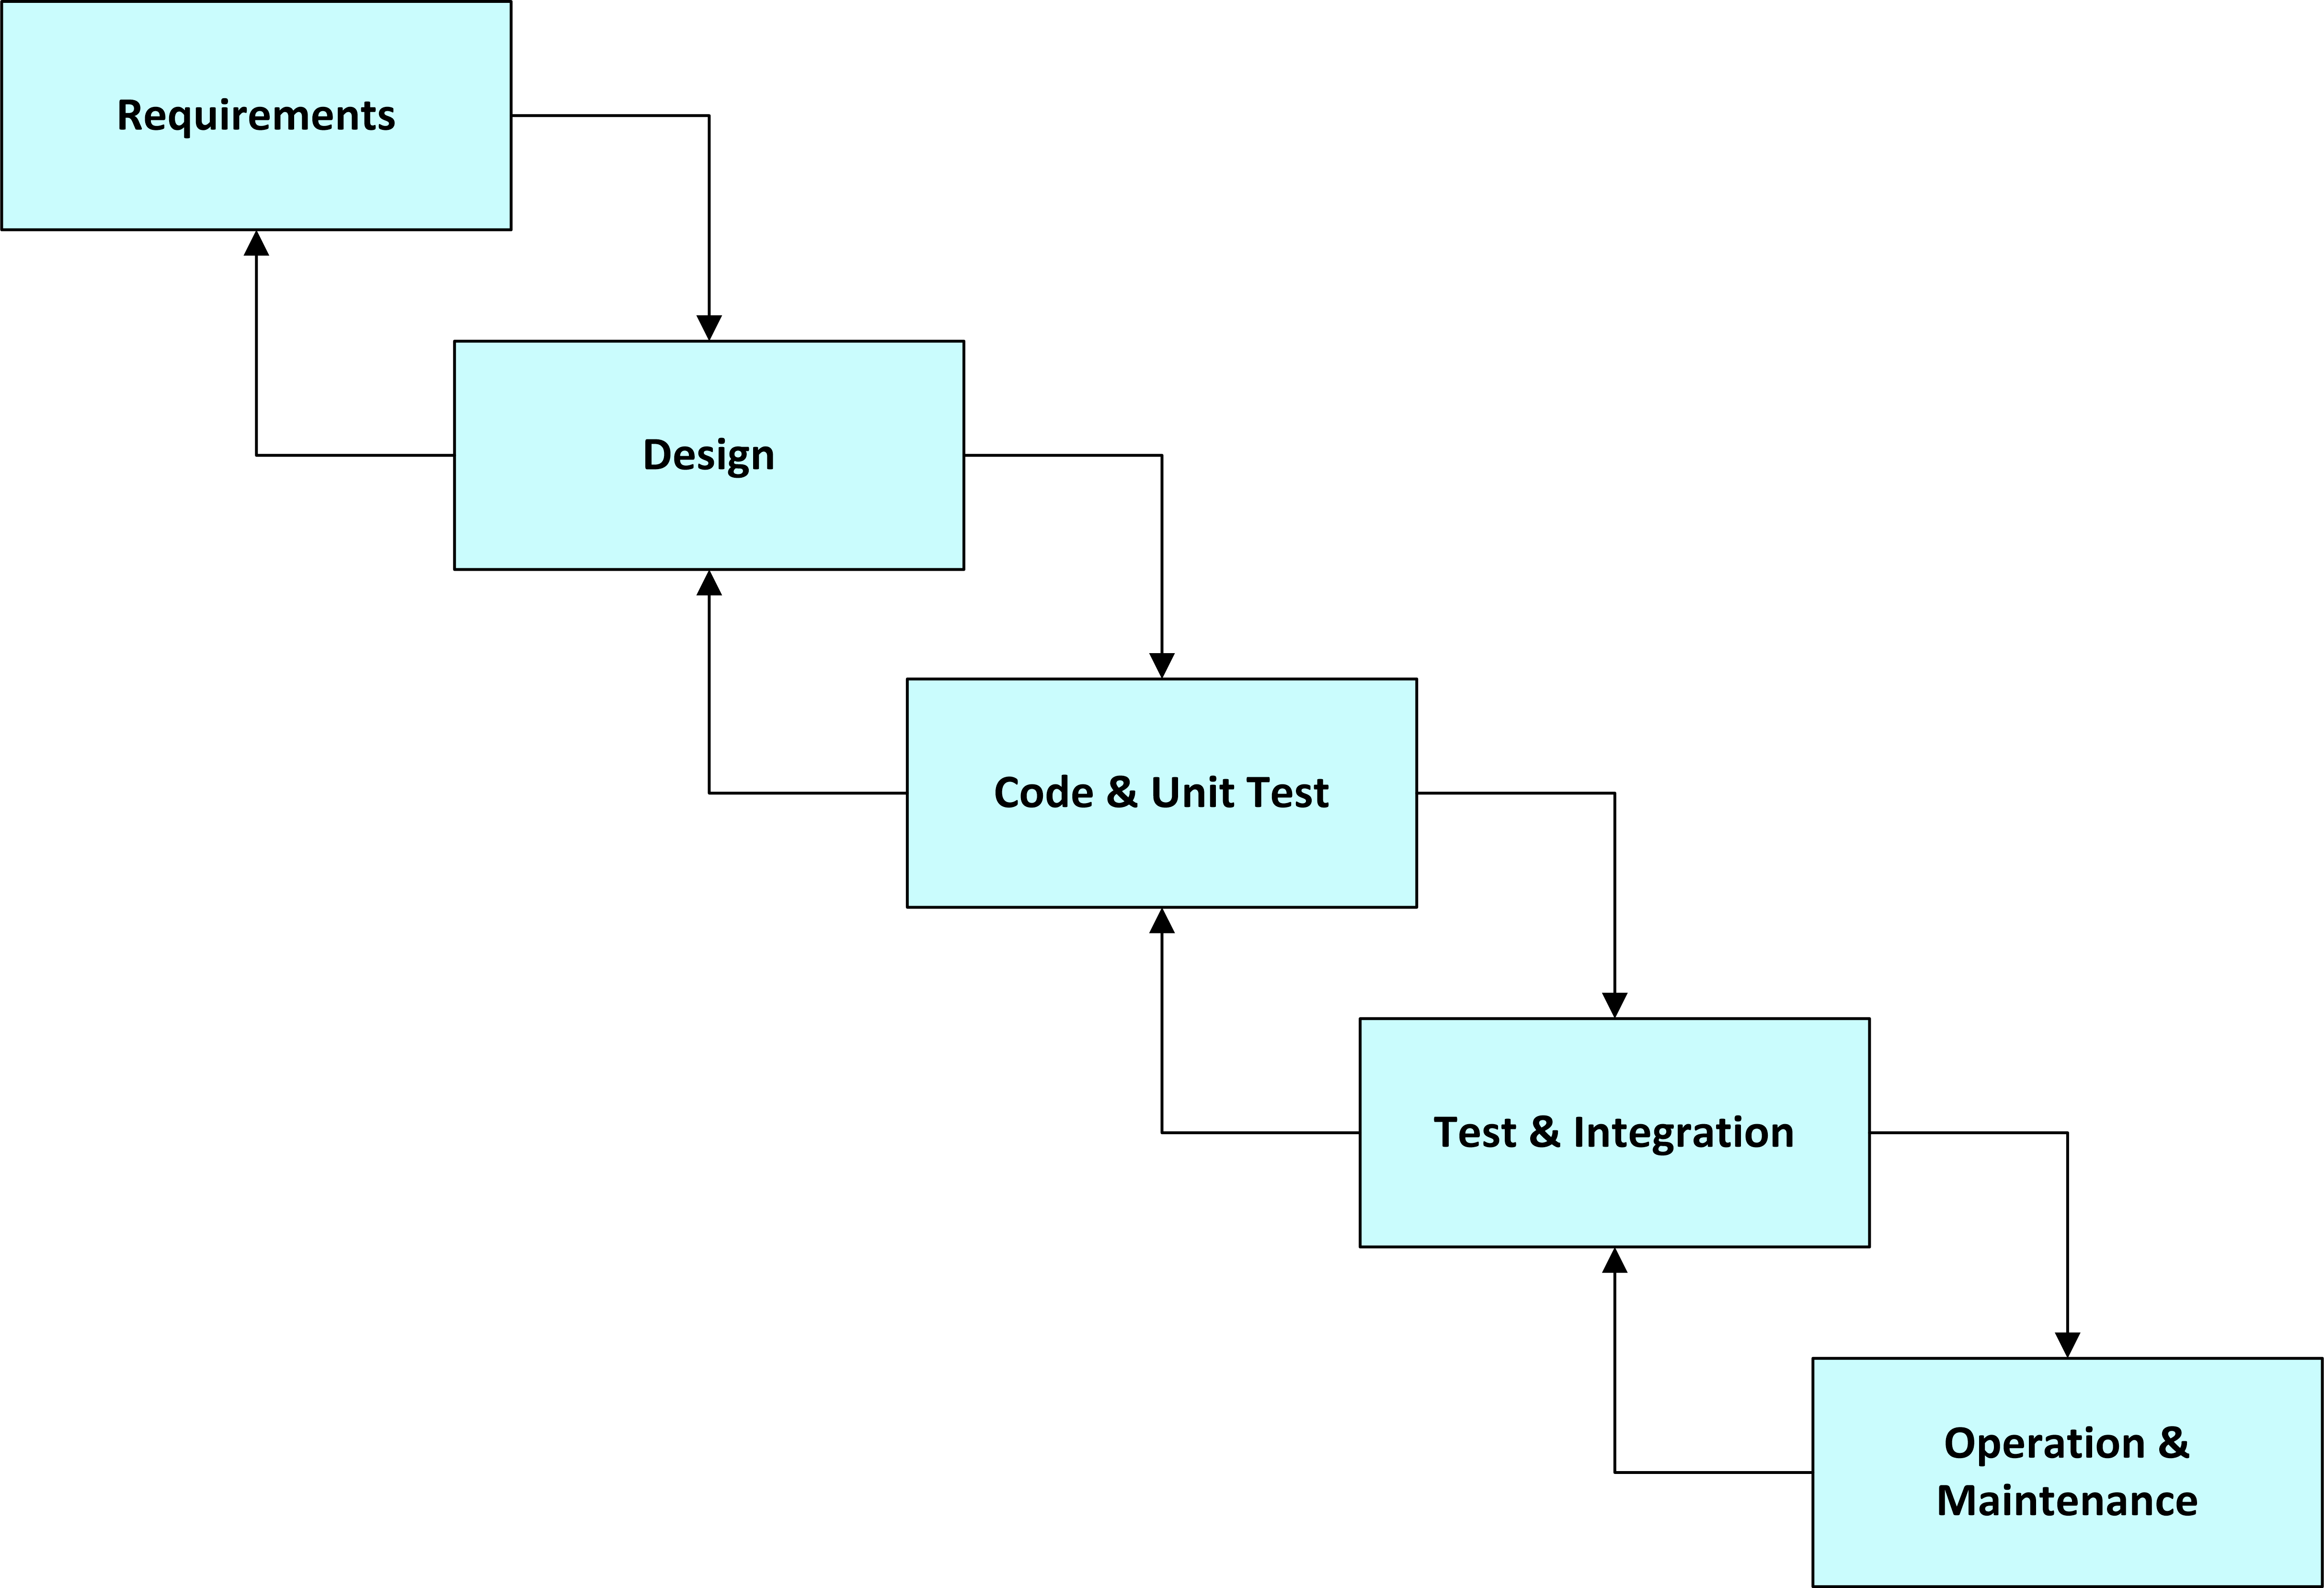
\includegraphics[scale=0.6]{chapter6/waterfall.png}
    \caption[Waterfall methodology]
      {Waterfall methodology highlighting the ``flow'' through the various 
      sections that make up a software development project.}
\end{figure}

\subsection{Advantages}
The waterfall model is the most commonly used methodology due to the following 
reasons \citep{alam:2012:Online}:
\begin{itemize}
	\item Documentation is produced at every stage, allowing for anyone to join
        the project at any time to have full understanding;
  \item Minimum resources are required to implement this model, and is simple
        to implement and follow;
  \item Testing is completed after every major stage of software development.
\end{itemize}

\subsection{Disadvantages}
However, the disadvantages of this methodology are \citep{alam:2012:Online}:
\begin{itemize}
	\item The model works well if there is no reverse flow. Reverse flow can 
        cause time delays;
  \item The model assumes that the client know exactly what they want, in 
        reality this is not the case;
  \item A working model of the software is not complete, until the end product 
        has been finished.
\end{itemize}